% !TeX root = it-governance-risk-compliance.tex
% !TeX encoding = UTF-8
\chapter{Keamanan Informasi: ISO/IEC 27001 dan NIST CSF 2.0}

\section*{Tujuan Pembelajaran}
\begin{itemize}
  \item Menjelaskan struktur ISMS (\textit{Information Security Management System}) menurut
  ISO/IEC 27001:2022 serta peran kontrol Annex A dan ISO/IEC 27002.
  \item Menyusun profil saat ini NIST CSF 2.0 untuk sebuah organisasi.
  \item Menganalisis celah kontrol keamanan dan mengaitkannya dengan skenario di \textit{risk
  register}.
\end{itemize}

\section{Pendahuluan}

Kebijakan keamanan Medikara sudah ditandatangani, tetapi audit internal masih menemukan akun
vendor tanpa batas waktu. Pengandaian pada bab sebelumnya memberi angkanya: 6 dari 30 akun sampel
masih aktif setelah penugasan berakhir, dan peninjauan bulan berikutnya mencabut 24 dari 120 akun.
Daftar yang diterima peninjau hanya memuat 108 akun, sehingga 12 akun luput. Dokumen kebijakan
menunjukkan niat. Organisasi tetap membutuhkan bukti bahwa petugas menyetujui akses, membatasi
kewenangan, dan mencabut akun ketika tugas selesai.

Medikara memiliki lima rumah sakit dengan versi Sistem Informasi Manajemen Rumah Sakit (SIMRS)
yang berbeda. Satu rumah sakit dapat menerapkan kontrol dengan baik, sementara lokasi lain belum
melakukannya. Penilaian karena itu harus menyebut cakupan sistem, lokasi, dan periode bukti. Hasil
kerja bab ini adalah profil keamanan saat ini dan daftar celah kontrol untuk tonggak C2 capstone.
Setiap celah ditautkan ke register risiko Bab 5 dan register kewajiban Bab 3.

Bab ini memakai ISO/IEC 27001:2022 sebagai persyaratan sistem manajemen, ISO/IEC 27002:2022
sebagai panduan kontrol, dan National Institute of Standards and Technology Cybersecurity
Framework (NIST CSF) 2.0 sebagai bahasa hasil keamanan. Penerapan pada organisasi kesehatan merujuk
ISO 27799:2025. ISO adalah International Organization for Standardization, dan IEC adalah
International Electrotechnical Commission. Naskah ISO berbayar, sehingga rincian klausulnya ditulis
ringkas dan perlu dicocokkan ke naskah berlisensi sebelum dipakai untuk audit. Publikasi NIST
terbuka dan dapat diperiksa mahasiswa. Seluruh angka tambahan tentang Medikara merupakan contoh
pembelajaran \cite{iso27001-2022,iso27002-2022,iso27799-2025,nistcsf2}.

\IfFileExists{../figures/ch06-diagram-konsep.png}{%

Gambar \ref{fig:ch06-ilustrasi-bab} merangkum hubungan komponen dan konsep utama bab ini.
\begin{figure}[!htb]
  \centering
  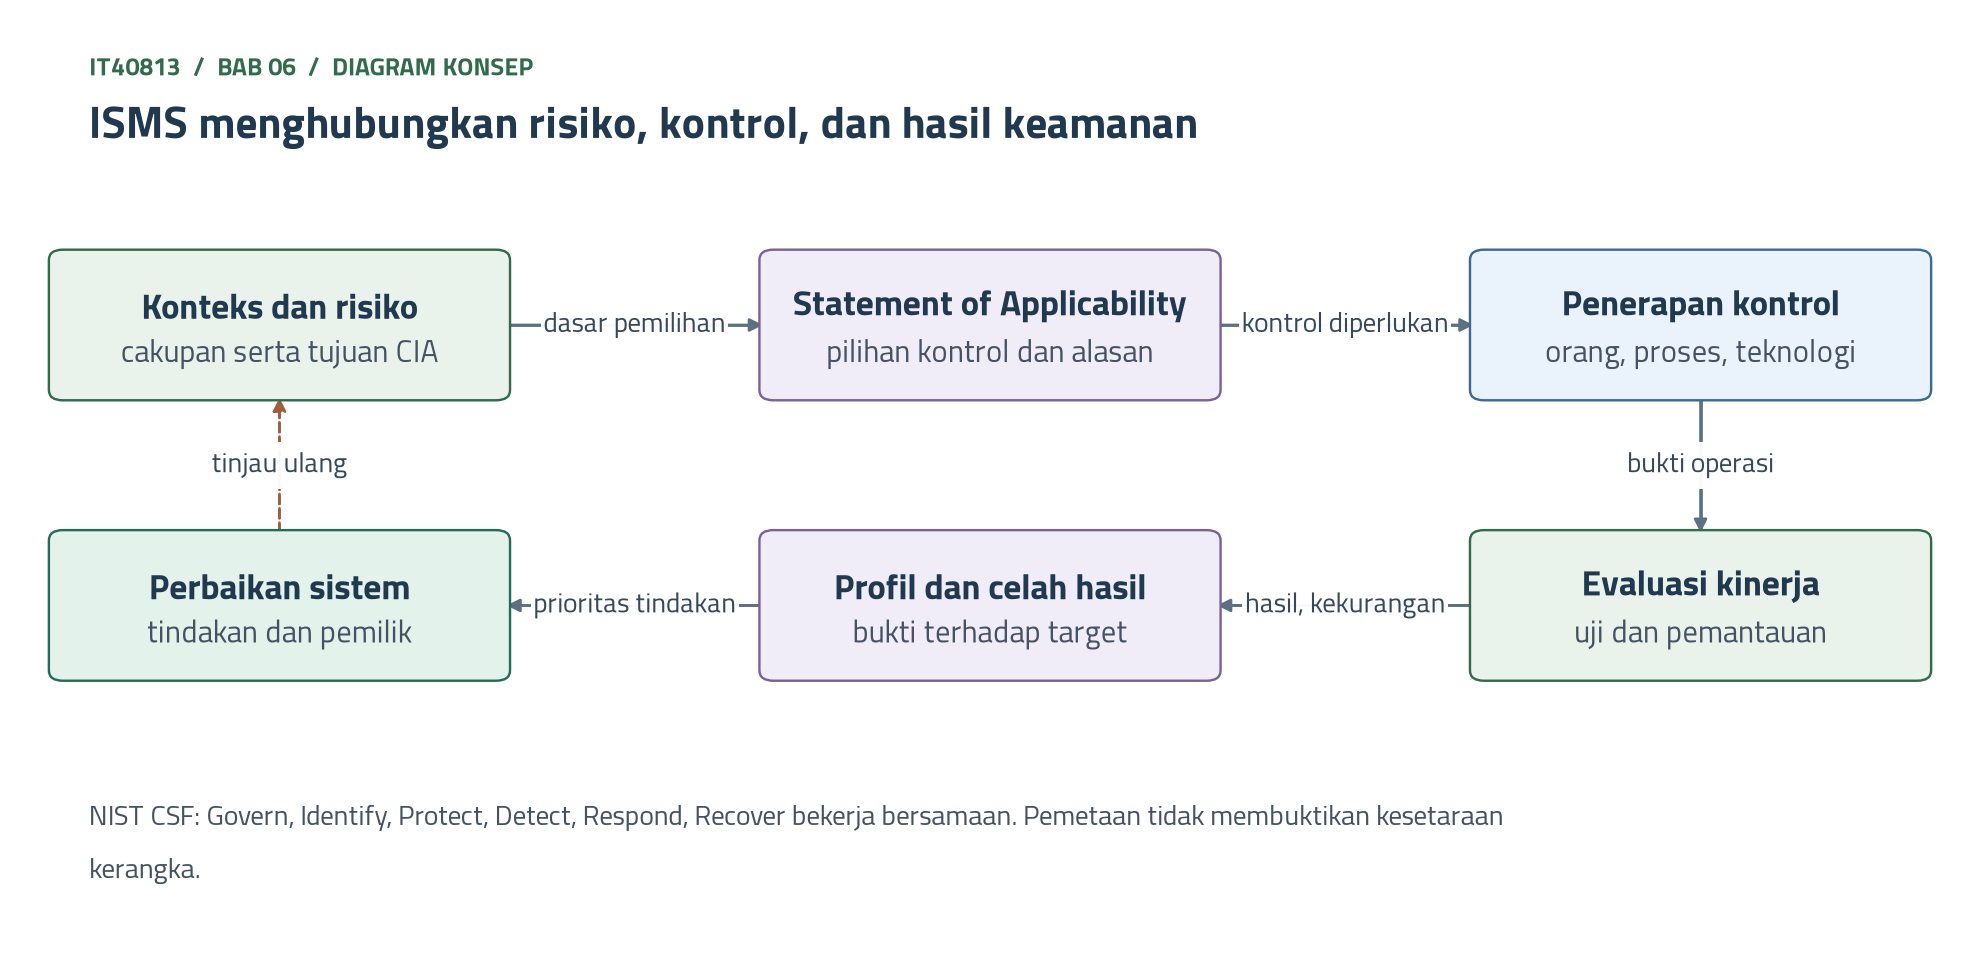
\includegraphics[width=\textwidth]{../figures/ch06-diagram-konsep.png}
  \caption{ISMS menghubungkan risiko, kontrol, dan hasil keamanan}
  \label{fig:ch06-ilustrasi-bab}
\end{figure}
}{}

\section{Kerahasiaan, Integritas, dan Ketersediaan}

\subsection*{Tiga tujuan pelindungan}

Keamanan informasi melindungi kerahasiaan, integritas, dan ketersediaan. Ketiganya sering disingkat
CIA, dari \textit{confidentiality}, \textit{integrity}, dan \textit{availability}. Kerahasiaan
membatasi siapa yang boleh membaca. Integritas menjaga ketepatan data serta perubahan yang sah.
Ketersediaan memastikan informasi dapat dipakai ketika diperlukan. Ketiga tujuan itu dapat saling
berbenturan, sehingga konfliknya diselesaikan sesuai konteks layanan.

Analogi lemari obat membantu menjelaskan pilihan. Lemari terkunci mengurangi akses yang tidak sah.
Pencatatan keluar masuk menjaga ketepatan stok. Kunci cadangan dan petugas pengganti menjaga
layanan ketika pemegang kunci utama tidak hadir.

Dua contoh memperlihatkan mengapa kontrol tidak cukup dinilai dari kerahasiaan:
\begin{enumerate}
  \item Misalkan satu akun bersama dipakai 12 petugas sebuah bangsal, dan dalam sebulan tercatat
  40 perubahan riwayat alergi. Sistem selalu tersedia dan tidak ada pihak luar yang membaca data.
  Namun, tidak satu pun dari 40 perubahan itu dapat ditelusuri kepada petugas tertentu.
  Kelemahannya ada pada integritas, dan kaitannya ada pada R-02 di register Bab 5.
  \item Misalkan semua akses darurat diblokir ketika pengelola identitas terganggu selama 2 jam.
  Data terlindung dari akses biasa, tetapi dokter tidak dapat membaca riwayat pengobatan. Bab 5
  menghitung gangguan 2 jam menyentuh sekitar 548 kunjungan. Akses darurat yang terbatas,
  beralasan, dan ditinjau menjadi pilihan yang perlu diuji.
\end{enumerate}

Tabel~\ref{tab:ch06-tiga-tujuan} merangkum tujuan pelindungan, pertanyaan layanan, dan bukti
contoh. Kode R-01, R-02, dan R-05 mengikuti register Bab 5.

\begin{table}[!htb]
  \centering\small
  \caption{Tujuan pelindungan dan bukti layanan}\label{tab:ch06-tiga-tujuan}
  \begin{tabularx}{\textwidth}{|>{\raggedright\arraybackslash}p{0.17\textwidth}|>{\raggedright\arraybackslash}X|>{\raggedright\arraybackslash}X|>{\raggedright\arraybackslash}p{0.09\textwidth}|}
    \hline
    \textbf{Tujuan} & \textbf{Pertanyaan} & \textbf{Bukti contoh} & \textbf{Risiko} \\ \hline
    Kerahasiaan & Apakah vendor hanya melihat data penugasannya? & Persetujuan dan pembatasan
    akses & R-01 \\ \hline
    Integritas & Siapa mengubah alergi dan kapan? & Jejak perubahan yang terlindungi & R-02 \\
    \hline
    Ketersediaan & Apakah data dapat dibaca saat gangguan? & Hasil uji pemulihan dan akses darurat
    & R-05 \\ \hline
  \end{tabularx}
\end{table}

\subsection*{Ketersediaan di rumah sakit: membaca satu penelitian}

Pertanyaan kemudian muncul: apakah gangguan ketersediaan di rumah sakit dapat diukur? Ghafur dan
rekan menelaah serangan \textit{ransomware} WannaCry 2017 pada National Health Service (NHS) Inggris
dengan data statistik episode rumah sakit \cite{c06-ghafur2019}. Penelitian itu memberi dua
pembacaan:
\begin{enumerate}
  \item Dampak terukur dalam layanan dan biaya. Pada 34 \textit{trust} rumah sakit yang terinfeksi,
  sekitar 13.500 janji rawat jalan dibatalkan pada pekan serangan. Pendaftaran gawat darurat turun
  sekitar 4 persen, dan pendaftaran elektif turun sekitar 9 persen, dihitung per hari per rumah
  sakit. Kerugian kegiatan diperkirakan £5,9 juta: £4 juta dari rawat inap, £0,6 juta dari gawat
  darurat, dan £1,3 juta dari rawat jalan.
  \item Satu ukuran tidak cukup. Penulis tidak menemukan kenaikan kematian, tetapi menyebut kematian
  sebagai ukuran kasar bagi bahaya terhadap pasien. Temuan itu tidak membuktikan serangan tanpa
  akibat klinis.
\end{enumerate}

Angka NHS tidak boleh disalin menjadi perkiraan kerugian Medikara, karena ukuran layanan dan sistem
pembiayaannya berbeda. Nilainya ada pada cara mengukur. Ketersediaan dinyatakan sebagai janji temu,
pendaftaran, dan biaya, bukan hanya jam server yang berhenti.

Dua hal juga sering tertukar: keamanan dan privasi. Pembagiannya begini. NIST menggambarkan
keduanya sebagai dua lingkaran yang beririsan \cite{nistcsf2}. Kebocoran lewat akun vendor berada
pada irisan itu. Pemakaian data yang sah secara teknis untuk tujuan lain dapat menjadi masalah
privasi tanpa insiden keamanan apa pun. Bab 7 merinci sisi pelindungan data pribadi.

\section{Sistem Manajemen ISO/IEC 27001}

\subsection*{Klausul 4 sampai 10}

Sistem manajemen keamanan informasi, atau ISMS, menghubungkan kebijakan, risiko, pelaksanaan,
evaluasi, dan perbaikan. ISO/IEC 27001 menetapkan persyaratan sistem manajemen itu. Klausul 4
sampai 10 mencakup konteks, kepemimpinan, perencanaan, dukungan, operasi, evaluasi kinerja, dan
perbaikan \cite{iso27001-2022}. Daftar alat dan kumpulan dokumen belum membentuk ISMS. Hubungan
antarbagian itulah yang diperiksa.

Analogi pengelolaan kebersihan dapur menunjukkan bedanya dengan daftar alat. Memiliki cairan
pembersih belum memastikan dapur bersih. Jadwal, pelaksana, pemeriksaan, penanganan kegagalan, dan
peninjauan pengelola membentuk sistem kerja.

Dua contoh membedakan kegiatan dan sistem:
\begin{enumerate}
  \item Misalkan tim membeli alat pemantauan untuk 5 rumah sakit. Tiap rumah sakit menghasilkan 300
  alarm per bulan, sehingga totalnya 1.500 alarm. Bila satu alarm ditelaah 10 menit, pekerjaannya
  250 jam per bulan, atau lebih dari satu orang penuh waktu dengan 160 jam kerja per bulan. Tanpa
  petugas, kriteria eskalasi, dan jadwal pemeriksaan, alarm hanya menjadi pesan yang menumpuk.
  Kekurangannya ada pada klausul dukungan dan operasi, bukan pada alat.
  \item Misalkan AC-01 dijalankan setiap bulan. Bulan pertama 24 dari 120 akun dicabut. Pemilik
  layanan membahas temuan itu dan menemukan sebabnya: tanggal berakhir penugasan tidak masuk
  daftar. Prosedur keluar vendor diubah, lalu jumlah pencabutan turun menjadi 9, 5, dan 2 akun pada
  tiga peninjauan berikutnya, atau turun sekitar 92 persen dari angka awal. Hubungan pelaksanaan,
  evaluasi, dan perbaikan menjadi terlihat.
\end{enumerate}

Gambar~\ref{fig:ch06-sistem} memperlihatkan urutan klausul tersebut. Gambar ini merupakan ringkasan
pembelajaran, bukan reproduksi isi standar. Singkatan SoA pada gambar berarti \textit{Statement of
Applicability}, yang dibahas pada seksi berikutnya. Tabel~\ref{tab:ch06-klausul} menerapkan tiap
klausul pada AC-01. Kode AC-01 mengikuti Bab 1, yaitu peninjauan akses berkala.

\begin{figure}[!htb]
  \centering
  \begin{tikzpicture}[
  font=\scriptsize,
  tahap/.style={draw, rounded corners, align=center, text width=2.35cm,
    minimum height=1.25cm, fill=blue!8},
  panah/.style={-{Stealth[length=2mm]}, thick}]
  \node[tahap, fill=praditagreen!15] (k4) at (0,0)
    {\textbf{Klausul 4}\\Konteks\\{\tiny\mdseries cakupan dan pihak terkait}};
  \node[tahap] (k5) at (3.05,0)
    {\textbf{Klausul 5}\\Kepemimpinan\\{\tiny\mdseries kebijakan dan peran}};
  \node[tahap] (k6) at (6.1,0)
    {\textbf{Klausul 6}\\Perencanaan\\{\tiny\mdseries risiko, SoA, sasaran}};
  \node[tahap] (k7) at (9.15,0)
    {\textbf{Klausul 7}\\Dukungan\\{\tiny\mdseries orang dan dokumen}};
  \node[tahap] (k8) at (9.15,-2.0)
    {\textbf{Klausul 8}\\Operasi\\{\tiny\mdseries kontrol dijalankan}};
  \node[tahap, fill=orange!12] (k9) at (6.1,-2.0)
    {\textbf{Klausul 9}\\Evaluasi kinerja\\{\tiny\mdseries uji, audit, tinjauan}};
  \node[tahap, fill=green!10] (k10) at (3.05,-2.0)
    {\textbf{Klausul 10}\\Perbaikan\\{\tiny\mdseries koreksi yang diverifikasi}};
  \draw[panah] (k4) -- (k5);
  \draw[panah] (k5) -- (k6);
  \draw[panah] (k6) -- (k7);
  \draw[panah] (k7) -- (k8);
  \draw[panah] (k8) -- (k9);
  \draw[panah] (k9) -- (k10);
  \draw[panah, dashed] (k10.west) -| node[pos=0.75, left, align=right]
    {tinjau\\ulang} (k4.south);
\end{tikzpicture}

  \caption{Klausul 4 sampai 10 sebagai satu sistem kerja}
  \label{fig:ch06-sistem}
\end{figure}

\begin{table}[!htb]
  \centering\small
  \caption{Klausul ISO/IEC 27001 pada kontrol AC-01 (misalkan)}\label{tab:ch06-klausul}
  \begin{tabularx}{\textwidth}{|>{\raggedright\arraybackslash}p{0.2\textwidth}|>{\raggedright\arraybackslash}X|>{\raggedright\arraybackslash}X|}
    \hline
    \textbf{Klausul} & \textbf{Pertanyaan} & \textbf{Bukti pada AC-01} \\ \hline
    4 Konteks & Sistem, lokasi, dan pihak mana yang masuk cakupan? & 5 rumah sakit, Medikara+, 120
    akun vendor; kewajiban K-01 \\ \hline
    5 Kepemimpinan & Siapa menetapkan kebijakan dan peran? & Kebijakan akses vendor; direksi
    menerima risiko sisa R-01 \\ \hline
    6 Perencanaan & Risiko dan kontrol apa yang dipilih? & R-01 dengan skor $3 \times 4 = 12$; baris
    SoA; sasaran nol akun tanpa pemilik \\ \hline
    7 Dukungan & Apakah orang dan dokumen cukup? & Peninjau yang ditunjuk; prosedur tertulis \\
    \hline
    8 Operasi & Apakah kontrol dijalankan? & Daftar akun, penandaan pemilik layanan, tiket
    pencabutan \\ \hline
    9 Evaluasi kinerja & Apakah kontrol bekerja? & 108 dari 120 akun tercakup; audit 6 dari 30 akun;
    tinjauan pimpinan \\ \hline
    10 Perbaikan & Apa yang berubah karena temuan? & Prosedur keluar vendor diubah; hasil diuji ulang
    \\ \hline
  \end{tabularx}
\end{table}

Keputusan membaca ISMS sebagai sistem punya dua konsekuensi. Pertama, temuan 12 akun yang luput
tidak ditutup hanya dengan mencabut 12 akun. Tim juga memeriksa mengapa daftar peninjau hanya memuat
108 akun. Kedua, kebijakan yang bagus tidak menaikkan penilaian bila catatan operasinya tidak ada.

Diagram konsep pada awal bab meringkas alur yang sama. Konteks dan risiko memberi dasar pemilihan
kontrol. SoA mencatat kontrol yang diperlukan. Penerapan kontrol menghasilkan bukti operasi. Evaluasi
kinerja menguji bukti itu, lalu hasil dan kekurangannya masuk ke profil dan celah hasil. Prioritas
tindakan menggerakkan perbaikan sistem, dan hasilnya ditinjau ulang.

Amandemen 1:2024 hanya mengubah dua subklausul. Rancangan adopsi Badan Standardisasi Nasional (BSN)
memuat teksnya. Subklausul 4.1 menambahkan kewajiban menentukan apakah perubahan iklim adalah isu
yang relevan. Subklausul 4.2 menambahkan catatan bahwa pihak berkepentingan dapat mempunyai
persyaratan terkait perubahan iklim \cite{c06-bsn-amd1}. Misalkan banjir musiman mengancam ruang
server satu rumah sakit. Tim mencatat hasil penentuan itu pada konteks ISMS, lalu menilai akibatnya
bersama R-05.

\subsection*{Sertifikat dan ruang lingkup}

Sertifikasi menilai sistem dalam ruang lingkup tertentu. Pertanyaan kemudian muncul: apa yang
dibuktikan sertifikat bagi Medikara? Bab 3 sudah menunjukkan sertifikat tidak menjawab kewajiban
hukum seperti dasar pemrosesan data. Dua contoh berikut menunjukkan batas lainnya:
\begin{enumerate}
  \item Misalkan Medikara memegang sertifikat untuk pusat data. Ke-36 fasilitas layanan, yaitu 5
  rumah sakit, 18 klinik, 1 laboratorium, dan 12 apotek, berada di luar ruang lingkup itu. Aplikasi
  vendor juga tidak otomatis tercakup.
  \item Misalkan vendor Medikara+ memiliki sertifikat yang masih berlaku 14 bulan, tetapi ruang
  lingkupnya hanya pengembangan aplikasi. Akun dukungan vendor yang masuk ke data pasien tidak
  termasuk. Masa berlaku yang panjang tidak menutup celah cakupan tersebut.
\end{enumerate}

Tanggal, penerbit, ruang lingkup, dan temuan karena itu tetap harus diperiksa sebelum sertifikat
dipakai sebagai bukti. Bab 9 memakai pemeriksaan yang sama untuk penyedia cloud.

Literatur ilmiah membantu membaca klaim manfaat sertifikasi. Tinjauan literatur Culot dan rekan
mengelompokkan penelitian ISO/IEC 27001 ke lima fokus: hubungan dengan standar lain, motivasi
penerapan, masalah saat penerapan, hasil yang mungkin, dan faktor konteks \cite{c06-culot2021}. Pada
pembacaan bab ini, susunan itu berguna sebagai daftar pertanyaan. Tim yang mendengar klaim ``sudah
bersertifikat'' dapat bertanya: mengapa sertifikat diambil, masalah apa yang muncul, dan hasil apa
yang benar-benar teramati.

\section{Annex A, SoA, dan Panduan Kontrol}

\subsection*{Annex A sebagai rujukan pemeriksa}

Annex A merupakan rujukan kontrol. Isinya 93 kontrol dalam empat tema: organisasi, manusia, fisik,
dan teknologi \cite{iso27001-2022,c06-dqs-annexa}. Berkas Informative References dari NIST
mencantumkan nomor yang sama: 5.1 sampai 5.37, 6.1 sampai 6.8, 7.1 sampai 7.14, dan 8.1 sampai 8.34
\cite{c06-nist-irefs}. \textit{Statement of Applicability} (SoA) menjelaskan kontrol yang diperlukan,
alasan pemilihan, status penerapan, dan alasan pengecualian kontrol Annex A yang tidak dipilih.
Annex A dipakai untuk memeriksa bahwa tidak ada kontrol perlu yang terlewat, bukan sebagai daftar
yang otomatis wajib seluruhnya.

Analogi daftar perlengkapan perjalanan menjelaskan pemilihan. Perjalanan pegunungan dan perjalanan
kota membutuhkan perlengkapan berbeda. Barang yang tidak dibawa harus dinilai terhadap tujuan dan
kondisi, bukan dihapus agar daftar terlihat lengkap.

Tabel~\ref{tab:ch06-tema} merangkum keempat tema. Uraian topik ditulis ringkas oleh bab ini dan
bukan terjemahan resmi. Nomor kontrol mengikuti berkas NIST tersebut.

\begin{table}[!htb]
  \centering\small
  \caption{Empat tema Annex A dan contoh topik pada Medikara}\label{tab:ch06-tema}
  \begin{tabularx}{\textwidth}{|>{\raggedright\arraybackslash}p{0.09\textwidth}|>{\raggedright\arraybackslash}p{0.17\textwidth}|>{\raggedright\arraybackslash}p{0.09\textwidth}|>{\raggedright\arraybackslash}X|}
    \hline
    \textbf{Nomor} & \textbf{Tema} & \textbf{Jumlah} & \textbf{Contoh topik pada Medikara} \\ \hline
    5 & Organisasi & 37 & 5.18 hak akses; 5.19 dan 5.20 hubungan serta perjanjian pemasok; 5.26
    tanggapan insiden \\ \hline
    6 & Manusia & 8 & Pelatihan petugas dan tanggung jawab setelah penugasan berakhir \\ \hline
    7 & Fisik & 14 & Ruang server dan perangkat di 36 fasilitas \\ \hline
    8 & Teknologi & 34 & 8.5 autentikasi; 8.13 cadangan; 8.15 pencatatan; 8.16 pemantauan \\ \hline
    Total & & 93 & \\ \hline
  \end{tabularx}
\end{table}

Dua hal pada keluarga standar ini sering tertukar: persyaratan dan panduan. Pembagiannya begini.
ISO/IEC 27001 berjudul \textit{Requirements} dan menjadi dasar penilaian sistem manajemen. ISO/IEC
27002 memberi panduan penerapan kontrol, sehingga tidak menjadi target sertifikasi sistem manajemen
tersendiri \cite{iso27001-2022,iso27002-2022}. ISO 27799:2025 memberi kontrol keamanan informasi
beserta panduan penerapan untuk organisasi kesehatan, dengan dasar ISO/IEC 27002 \cite{iso27799-2025}.
Tabel~\ref{tab:ch06-standar} membandingkan ketiganya.

\begin{table}[!htb]
  \centering\small
  \caption{Tiga standar dan pemakaiannya pada Medikara}\label{tab:ch06-standar}
  \begin{tabularx}{\textwidth}{|>{\raggedright\arraybackslash}p{0.2\textwidth}|>{\raggedright\arraybackslash}p{0.24\textwidth}|>{\raggedright\arraybackslash}X|}
    \hline
    \textbf{Standar} & \textbf{Sifat} & \textbf{Pemakaian pada Medikara} \\ \hline
    ISO/IEC 27001:2022 & Persyaratan sistem manajemen & Menilai ruang lingkup ISMS, SoA, evaluasi,
    dan perbaikan \\ \hline
    ISO/IEC 27002:2022 & Panduan penerapan kontrol & Menjelaskan cara merancang peninjauan hak akses
    pada AC-01 \\ \hline
    ISO 27799:2025 & Panduan kontrol untuk organisasi kesehatan & Membaca kontrol untuk rekam medis
    elektronik, perangkat digital fasilitas, dan telekonsultasi Medikara+ \\ \hline
  \end{tabularx}
\end{table}

\subsection*{Dari risiko ke SoA}

Pertanyaan berikutnya: dari mana kontrol dalam SoA berasal? Dari penanganan risiko. Tim memilih
penanganan, menetapkan kontrol yang diperlukan, lalu membandingkannya dengan Annex A.
Gambar~\ref{fig:ch06-rantai-soa} memperlihatkan rantai itu untuk R-01. Hasilnya berupa bukti operasi
yang dapat diuji.

\begin{figure}[!htb]
  \centering
  \begin{tikzpicture}[
  font=\scriptsize,
  tahap/.style={draw, rounded corners, align=center, text width=3.0cm,
    minimum height=1.1cm, fill=blue!8},
  panah/.style={-{Stealth[length=2mm]}, thick}]
  \node[tahap, fill=praditagreen!15] (risiko) at (0,0)
    {\textbf{Risiko R-01}\\{\tiny\mdseries skor $3 \times 4 = 12$, dinilai pada Bab 5}};
  \node[tahap] (tangani) at (4.1,0)
    {\textbf{Penanganan dipilih}\\{\tiny\mdseries kurangi paparan akun vendor}};
  \node[tahap] (perlu) at (8.2,0)
    {\textbf{Kontrol diperlukan}\\{\tiny\mdseries AC-01 dan pemantauan aktivitas}};
  \node[tahap] (banding) at (8.2,-1.9)
    {\textbf{Dibandingkan dengan Annex A}\\{\tiny\mdseries 93 kontrol sebagai rujukan}};
  \node[tahap, fill=orange!12] (soa) at (4.1,-1.9)
    {\textbf{SoA}\\{\tiny\mdseries kontrol, alasan, status, pengecualian}};
  \node[tahap, fill=green!10] (bukti) at (0,-1.9)
    {\textbf{Bukti operasi}\\{\tiny\mdseries daftar akun, keputusan, tiket pencabutan}};
  \draw[panah] (risiko) -- (tangani);
  \draw[panah] (tangani) -- (perlu);
  \draw[panah] (perlu) -- (banding);
  \draw[panah] (banding) -- (soa);
  \draw[panah] (soa) -- (bukti);
  \draw[panah, dashed] (bukti) -- node[right, align=left] {tinjau ulang} (risiko);
\end{tikzpicture}

  \caption{Rantai dari risiko ke SoA dan bukti operasi}
  \label{fig:ch06-rantai-soa}
\end{figure}

Dua contoh menguji alasan pemilihan:
\begin{enumerate}
  \item Misalkan akses vendor diperlukan untuk perbaikan. AC-01 dipilih karena R-01 dan K-01. Bukti
  mencakup daftar hak akses, peninjau yang sah, hasil keputusan, dan pencabutan. Status pada SoA
  ditulis ``diterapkan sebagian'', karena 12 dari 120 akun luput dan bukti peninjauan baru ada pada
  1 dari 5 rumah sakit.
  \item Misalkan Medikara tidak mengembangkan satu aplikasi sendiri, lalu mengusulkan pengecualian
  kontrol pengembangan. Sekitar 28.000 janji temu per bulan berjalan pada Medikara+ buatan vendor,
  dan R-07 menyebut perubahan yang tidak diuji. Pengadaan dan perubahan oleh vendor tetap menimbulkan
  kebutuhan kontrol, misalnya 8.30 tentang pengembangan alih daya dan 8.32 tentang manajemen
  perubahan. Usulan itu belum dapat diterima.
\end{enumerate}

Tabel~\ref{tab:ch06-soa} merangkum penalaran SoA tersebut sebagai ringkasan pembelajaran. Berkas
\berkas{sources/chapter06/catatan-soa.md} menyediakan lembar isiannya.

\begin{table}[!htb]
  \centering\small
  \caption{Contoh penalaran SoA (ringkasan pembelajaran)}\label{tab:ch06-soa}
  \begin{tabularx}{\textwidth}{|>{\raggedright\arraybackslash}p{0.25\textwidth}|>{\raggedright\arraybackslash}X|>{\raggedright\arraybackslash}X|}
    \hline
    \textbf{Kontrol} & \textbf{Alasan} & \textbf{Status dan bukti} \\ \hline
    Peninjauan hak akses, AC-01 (Annex A 5.18) & Mengurangi akses vendor berlebih pada R-01;
    mendukung K-01 & Diterapkan sebagian; bukti baru 1 dari 5 rumah sakit \\ \hline
    Pencatatan aktivitas (Annex A 8.15) & Menelusuri perubahan data pada R-01 dan R-02 & Catatan ada;
    perlindungan dan tinjauan belum terbukti \\ \hline
    Cadangan dan pemulihan (Annex A 8.13) & Menjaga data saat gangguan pada R-05; mendukung K-02 &
    Cadangan tersedia; hasil uji pemulihan diminta \\ \hline
    Pengembangan alih daya (Annex A 8.30) & Vendor mengubah Medikara+; R-07 & Usulan pengecualian
    ditolak; kontrol dinilai pada kontrak vendor \\ \hline
  \end{tabularx}
\end{table}

Keputusan mengecualikan kontrol punya dua konsekuensi. Pertama, alasannya harus dapat diuji
peninjau, sehingga kalimat ``tidak relevan'' saja tidak cukup. Kedua, pengecualian perlu ditinjau
ulang ketika cakupan berubah. Skenario Bab 4 menambah dua fasilitas, dari 36 menjadi 38, sehingga
baris yang menyangkut lokasi harus dibaca ulang.

Kode juga sering tertukar. AC-01 pada bab ini adalah kode lokal Medikara. Angka 5.18 adalah nomor
kontrol Annex A. Berkas NIST juga memuat label AC-01 milik NIST Special Publication (SP) 800-53 pada
subkategori PR.AA-05 \cite{c06-nist-irefs}, dan label itu bukan kontrol Medikara. Register sebaiknya
selalu menulis sumber kode, supaya pembaca tidak menganggap ketiganya satu kontrol yang sama.

\subsection*{Konteks kesehatan}

Cakupan ISO 27799:2025 meliputi perangkat lunak kesehatan seperti sistem rekam medis elektronik, dan
perangkat medis yang mengandung perangkat lunak. Standar itu berlaku pada organisasi kesehatan dari
segala jenis dan ukuran, termasuk layanan jarak jauh \cite{iso27799-2025}. Medikara dengan 36
fasilitas dan telekonsultasi berada dalam gambaran itu. Penilaian karena itu melibatkan pimpinan
klinis. Pembatasan akses tidak boleh merusak kebutuhan pelayanan darurat. NIST juga mencontohkan
akses darurat pada PR.AA-03: petugas yang berwenang tetap dapat mengakses akun yang penting bagi
keselamatan \cite{c06-nist-irefs}. Persetujuan pengecualian dan peninjauan setelah kejadian tetap
diperlukan.

Bab 5 sudah membatasi pengecualian darurat pada akun vendor paling lama 24 jam. Misalkan dalam
sebulan terjadi 6 pengecualian seperti itu pada 120 akun. Keenamnya ditinjau pemilik layanan pada
hari kerja berikutnya. Bila hanya 4 yang punya catatan alasan, kontrol bukan berjalan 67 persen,
melainkan ada 2 pengecualian yang tidak dapat dipertanggungjawabkan.

\begin{kasus}[title={Kasus Medikara Health: Menyusun SoA untuk Cakupan Terbatas}]
Misalkan tim menilai 93 kontrol untuk cakupan 5 rumah sakit dan Medikara+. Hasil awalnya 84 kontrol
diperlukan dan 9 kontrol diusulkan dikecualikan, atau sekitar 9,7 persen. Peninjau menguji kesembilan
usulan dengan register Bab 5. Tiga usulan ditolak karena R-07 menunjukkan vendor tetap mengubah
Medikara+. Hasil akhirnya 87 kontrol diperlukan dan 6 dikecualikan.

Keputusan ini punya dua konsekuensi. Pertama, pekerjaan bertambah 3 baris yang harus punya pemilik
dan bukti. Kedua, keenam pengecualian tersisa ditulis dengan alasan, pihak yang menyetujui, dan
tanggal tinjau ulang. Jumlah kontrol yang diperlukan bukan ukuran keamanan. Kualitas alasannya yang
dinilai.
\end{kasus}

\section{Enam Fungsi NIST CSF 2.0}

\subsection*{Struktur inti}

NIST CSF 2.0 menyusun hasil keamanan dalam hierarki fungsi, kategori, dan subkategori. Hitungan bab
ini pada lampiran naskahnya menghasilkan 6 fungsi, 22 kategori, dan 106 subkategori. Enam fungsinya
adalah Govern, Identify, Protect, Detect, Respond, dan Recover. Hasil itu bukan daftar periksa
tindakan. Urutannya juga tidak menyatakan urutan kerja atau tingkat kepentingan. Fungsi perlu
ditangani bersamaan. Kerangka ini menjelaskan hasil yang diinginkan tanpa menetapkan cara
mencapainya \cite{nistcsf2}.

Analogi pengamanan gedung menunjukkan hubungan antarfungsi. Pengelola menetapkan aturan, mendata
ruangan, memasang pengamanan, mendeteksi gangguan, menanganinya, lalu memulihkan penggunaan. Pintu
yang kuat tidak menggantikan petugas dan rencana penanganan.

Gambar~\ref{fig:ch06-enam-fungsi} menempatkan Govern di tengah, karena fungsi itu menjadi dasar cara
lima fungsi lain dijalankan. Gambar ini digambar ulang untuk bab ini.
Tabel~\ref{tab:ch06-fungsi} merangkum hasil tiap fungsi dan pertanyaan bagi Medikara.

\begin{figure}[!htb]
  \centering
  \begin{tikzpicture}[
  font=\scriptsize,
  fungsi/.style={draw, rounded corners, align=center, text width=2.2cm,
    minimum height=0.95cm, fill=blue!8},
  panah/.style={-{Stealth[length=2mm]}, thick}]
  \node[fungsi, fill=praditagreen!15, text width=2.7cm, minimum height=1.2cm] (gv) at (0,0)
    {\textbf{Govern}\\{\tiny\mdseries arah, peran, kebijakan, pengawasan, pemasok}};
  \node[fungsi] (id) at (0,2.3) {\textbf{Identify}\\{\tiny\mdseries aset, risiko, perbaikan}};
  \node[fungsi] (pr) at (4.2,0.8) {\textbf{Protect}\\{\tiny\mdseries akses, data, platform}};
  \node[fungsi] (de) at (2.55,-2.0) {\textbf{Detect}\\{\tiny\mdseries pemantauan, analisis}};
  \node[fungsi] (rs) at (-2.55,-2.0) {\textbf{Respond}\\{\tiny\mdseries insiden, komunikasi}};
  \node[fungsi] (rc) at (-4.2,0.8) {\textbf{Recover}\\{\tiny\mdseries pemulihan, komunikasi}};
  \draw[gray, thin] (id) -- (pr) -- (de) -- (rs) -- (rc) -- (id);
  \draw[panah] (gv) -- (id);
  \draw[panah] (gv) -- (pr);
  \draw[panah] (gv) -- (de);
  \draw[panah] (gv) -- (rs);
  \draw[panah] (gv) -- (rc);
\end{tikzpicture}

  \caption{Govern mengarahkan lima fungsi lain yang saling berhubungan}
  \label{fig:ch06-enam-fungsi}
\end{figure}

\begin{table}[!htb]
  \centering\small
  \caption{Hasil dan pertanyaan penilaian pada enam fungsi}\label{tab:ch06-fungsi}
  \begin{tabularx}{\textwidth}{|>{\raggedright\arraybackslash}p{0.14\textwidth}|>{\raggedright\arraybackslash}X|>{\raggedright\arraybackslash}X|>{\raggedright\arraybackslash}p{0.23\textwidth}|}
    \hline
    \textbf{Fungsi} & \textbf{Hasil (ringkasan)} & \textbf{Pertanyaan Medikara} & \textbf{Bukti contoh}
    \\ \hline
    Govern & Strategi, harapan, dan kebijakan risiko ditetapkan serta dipantau & Siapa menerima
    risiko akses vendor? & Keputusan dan wewenang \\ \hline
    Identify & Risiko keamanan saat ini dipahami & Sistem dan data apa yang terlibat? & Inventaris
    serta alur data \\ \hline
    Protect & Pengaman dipakai untuk mengelola risiko & Bagaimana akses dibatasi? & Daftar hak dan
    bukti AC-01 \\ \hline
    Detect & Kemungkinan serangan ditemukan dan dianalisis & Bagaimana akses menyimpang diketahui? &
    Catatan alarm dan tinjauan \\ \hline
    Respond & Tindakan atas insiden yang terdeteksi diambil & Siapa membekukan akses? & Prosedur dan
    hasil latihan \\ \hline
    Recover & Aset dan operasi yang terdampak dipulihkan & Bagaimana data dipulihkan? & Hasil uji
    pemulihan \\ \hline
  \end{tabularx}
\end{table}

Dua contoh menunjukkan fungsi yang saling melengkapi:
\begin{enumerate}
  \item Misalkan seluruh 108 akun pada daftar peninjau memakai Multi-Factor Authentication (MFA).
  Cakupannya tampak 100 persen. Terhadap populasi 120 akun, cakupannya hanya 90 persen, karena 12
  akun tidak tercatat. Protect yang kuat tidak menolong bila Identify belum lengkap.
  \item Misalkan alarm akses diterima dalam 5 menit. Tanpa petugas yang berwenang membekukan akun,
  kecepatan deteksi belum menghasilkan penanganan. Data latihan Bab 1 memberi pembandingnya: akun
  dukungan memanggil data selama 8 malam dan baru diketahui pada hari ke-11.
\end{enumerate}

Inventaris pada ID.AM-02 juga mencakup layanan \textit{Application Programming Interface} (API) dan
layanan cloud \cite{c06-nist-irefs}. Bab ini cukup memastikan keduanya masuk cakupan profil. Cara
mengamankan API dibahas pada mata kuliah IT40613, dan keamanan cloud pada IT40713.

\subsection*{Mengapa Govern ditambahkan}

Versi 1.1 memiliki lima fungsi: Identify, Protect, Detect, Respond, dan Recover
\cite{c06-nist-csf11}. Versi 2.0 menambahkan Govern dan menonjolkan tata kelola serta rantai pasok
\cite{nistcsf2}. Masalah organisasi apa yang ingin diselesaikan? NIST menulis bahwa kegiatan tata
kelola penting untuk memasukkan keamanan ke strategi risiko enterprise, dan bahwa pimpinan
mengomunikasikan harapan tentang \textit{risk appetite}, akuntabilitas, dan sumber daya. Tanpa fungsi
ini, penilaian keamanan mudah berhenti sebagai urusan tim teknis. Kalimat terakhir merupakan
penafsiran bab ini.

Tabel~\ref{tab:ch06-govern} menautkan kategori Govern dengan hasil kerja bab sebelumnya. Enam
kategori pada Govern adalah konteks organisasi (GV.OC), strategi pengelolaan risiko (GV.RM), peran
dan wewenang (GV.RR), kebijakan (GV.PO), pengawasan (GV.OV), dan pengelolaan risiko rantai pasok
(GV.SC).

\begin{table}[!htb]
  \centering\small
  \caption{Subkategori Govern dan hasil kerja bab sebelumnya}\label{tab:ch06-govern}
  \begin{tabularx}{\textwidth}{|>{\raggedright\arraybackslash}p{0.14\textwidth}|>{\raggedright\arraybackslash}X|>{\raggedright\arraybackslash}X|}
    \hline
    \textbf{Subkategori} & \textbf{Hasil (ringkasan)} & \textbf{Hasil kerja Medikara} \\ \hline
    GV.OC-03 & Persyaratan hukum, regulasi, dan kontrak dipahami serta dikelola & Register K-01
    sampai K-16 pada Bab 3 \\ \hline
    GV.RM-02 & Pernyataan \textit{risk appetite} dan \textit{risk tolerance} ditetapkan & Batas nol
    akun vendor aktif tanpa pemilik pada Bab 5 \\ \hline
    GV.RR-02 & Peran, tanggung jawab, dan wewenang ditetapkan serta ditegakkan & Hak keputusan akses
    vendor pada Bab 2 \\ \hline
    GV.SC-07 & Risiko pemasok dipahami dan dipantau sepanjang hubungan & Vendor Medikara+, R-01, dan
    insiden 2025 \\ \hline
  \end{tabularx}
\end{table}

\subsection*{ISO/IEC 27001 dan NIST CSF}

Dua kerangka ini juga sering tertukar. Pembagiannya begini. ISO/IEC 27001 menetapkan persyaratan yang
dapat dinilai dalam ruang lingkup tertentu. NIST CSF menyediakan bahasa hasil yang dapat dipakai
secara sukarela atau lewat kebijakan pemerintah, dan naskah 2.0 tidak memuat skema sertifikasi
\cite{nistcsf2}. Tabel~\ref{tab:ch06-iso-csf} menunjukkan bahwa keduanya melengkapi, bukan
menggantikan.

\begin{table}[!htb]
  \centering\small
  \caption{Perbedaan ISO/IEC 27001 dan NIST CSF 2.0}\label{tab:ch06-iso-csf}
  \begin{tabularx}{\textwidth}{|>{\raggedright\arraybackslash}p{0.17\textwidth}|>{\raggedright\arraybackslash}X|>{\raggedright\arraybackslash}X|}
    \hline
    \textbf{Pembeda} & \textbf{ISO/IEC 27001:2022} & \textbf{NIST CSF 2.0} \\ \hline
    Sifat & Persyaratan sistem manajemen & Taksonomi hasil, tanpa menetapkan cara \\ \hline
    Unsur & Klausul 4 sampai 10, 93 kontrol Annex A, SoA & 6 fungsi, 22 kategori, 106 subkategori,
    profil, \textit{tier} \\ \hline
    Pemeriksaan & Dapat disertifikasi dalam ruang lingkup & Tidak ada skema sertifikasi pada naskah
    2.0 \\ \hline
    Akses naskah & Berbayar & Terbuka \\ \hline
    Luaran Medikara & Ruang lingkup ISMS, SoA, hasil evaluasi & Profil saat ini, celah, profil target
    Bab 8 \\ \hline
  \end{tabularx}
\end{table}

\section{Profil Saat Ini dan Tier}

\subsection*{Profil organisasi}

Profil organisasi menggambarkan keadaan keamanan saat ini atau target dalam bahasa hasil pada CSF.
Profil saat ini (\textit{Current Profile}) menyebut hasil yang sedang dicapai dan seberapa jauh hasil
itu tercapai. Profil target (\textit{Target Profile}) menyebut hasil yang dipilih dan diprioritaskan
\cite{nistcsf2}. Satu organisasi dapat memiliki beberapa profil, masing-masing dengan cakupan berbeda.
Setiap kesimpulan memerlukan bukti dan catatan batasnya.

Analogi potret cabang toko menunjukkan pentingnya cakupan. Foto satu rak yang rapi tidak menunjukkan
seluruh toko. Potret harus menjelaskan rak, tanggal, dan bagian yang tidak terlihat.

NIST menyarankan lima langkah: menetapkan cakupan, mengumpulkan informasi, membuat profil,
menganalisis celah serta menyusun rencana tindakan, lalu menjalankan rencana dan memperbarui profil
\cite{nistcsf2,c06-nist-sp1301}. Gambar~\ref{fig:ch06-langkah-profil} menerapkannya pada Medikara.
Templat NIST memuat kolom praktik, status, peringkat, prioritas, dan sasaran, dan kolom itu boleh
disesuaikan \cite{c06-nist-sp1301}. Bab ini mengerjakan langkah 1 sampai 4 untuk profil saat ini.
Profil target dirancang pada Bab 8.

\begin{figure}[!htb]
  \centering
  \begin{tikzpicture}[
  font=\scriptsize,
  tahap/.style={draw, rounded corners, align=center, text width=1.9cm,
    minimum height=1.0cm, fill=blue!8},
  hasil/.style={draw, align=center, text width=1.9cm, minimum height=1.05cm,
    fill=white, font=\tiny},
  panah/.style={-{Stealth[length=2mm]}, thick}]
  \node[tahap] (s1) at (0,0) {1. Tetapkan cakupan};
  \node[tahap] (s2) at (2.45,0) {2. Kumpulkan informasi};
  \node[tahap, fill=orange!12] (s3) at (4.9,0) {3. Buat profil};
  \node[tahap, fill=orange!12] (s4) at (7.35,0) {4. Analisis celah dan rencana};
  \node[tahap, fill=green!10] (s5) at (9.8,0) {5. Jalankan dan perbarui};
  \node[hasil] (h1) at (0,-1.55) {5 rumah sakit, Medikara+, 120 akun, 12 bulan};
  \node[hasil] (h2) at (2.45,-1.55) {Register Bab 3, register Bab 5, sumber bukti};
  \node[hasil] (h3) at (4.9,-1.55) {14 subkategori dengan status lokal};
  \node[hasil] (h4) at (7.35,-1.55) {6 celah, 3 prioritas untuk Bab 8};
  \node[hasil] (h5) at (9.8,-1.55) {Profil target Bab 8, tonggak C3};
  \draw[panah] (s1) -- (s2);
  \draw[panah] (s2) -- (s3);
  \draw[panah] (s3) -- (s4);
  \draw[panah] (s4) -- (s5);
  \foreach \nomor in {1,2,3,4,5} {
    \draw[gray, thin] (s\nomor) -- (h\nomor);
  }
  \draw[panah, dashed] (s5.north) -- ++(0,0.4) -| node[pos=0.25, above] {ulangi} (s1.north);
\end{tikzpicture}

  \caption{Lima langkah membuat dan memakai profil, dengan keluaran Medikara (misalkan)}
  \label{fig:ch06-langkah-profil}
\end{figure}

Dua contoh menguji kualitas klaim:
\begin{enumerate}
  \item Audit Bab 4 memeriksa 30 akun, dan 24 di antaranya sesuai, atau 80 persen. Tim menyimpulkan
  ada 6 pengecualian dalam sampel. Tim tidak menyatakan seluruh organisasi 80 persen aman. Angka 24
  dari 120 akun berasal dari peninjauan penuh, bukan dari proyeksi sampel. Daftarnya pun hanya memuat
  108 akun dan buktinya hanya ada pada 1 dari 5 rumah sakit.
  \item Misalkan cadangan berhasil dibuat setiap malam selama 30 hari pada 5 rumah sakit, sehingga
  ada 150 pekerjaan cadangan yang berhasil. Tim belum menyatakan pemulihan tercapai sebelum data
  dipulihkan dan pemilik layanan menguji kelengkapannya. PR.DS-11 meminta cadangan juga diuji, dan
  RC.RP-03 meminta integritas cadangan diverifikasi sebelum dipakai \cite{nistcsf2}.
\end{enumerate}

Tabel~\ref{tab:ch06-profil} merangkum status lokal yang dipakai tim. Daftar ini merupakan alat kerja
bab ini, bukan skala resmi NIST. NIST memberi contoh skala seperti tinggi, sedang, dan rendah, atau
1 sampai 5 \cite{c06-nist-sp1301}. Status lokal dipilih karena memisahkan ``belum terbukti'' dari
``gagal''.

\begin{table}[!htb]
  \centering\small
  \caption{Status lokal yang dipakai tim}\label{tab:ch06-profil}
  \begin{tabularx}{\textwidth}{|>{\raggedright\arraybackslash}p{0.2\textwidth}|>{\raggedright\arraybackslash}X|>{\raggedright\arraybackslash}X|}
    \hline
    \textbf{Status lokal} & \textbf{Arti} & \textbf{Tindakan} \\ \hline
    Terbukti & Bukti sesuai cakupan dan periode & Simpan sumber dan peninjau \\ \hline
    Sebagian & Sebagian hasil atau lokasi belum tercakup & Jelaskan celah spesifik \\ \hline
    Belum ada bukti & Klaim belum dapat diuji & Minta bukti; jangan beri status lulus \\ \hline
    Tidak relevan & Ada alasan terhadap cakupan & Catat persetujuan dan tinjau ulang \\ \hline
  \end{tabularx}
\end{table}

\subsection*{Contoh profil saat ini}

Misalkan tim Medikara memilih cakupan akses vendor dan SIMRS pada 5 rumah sakit serta Medikara+,
untuk periode 12 bulan. Tim memilih 14 dari 106 subkategori, atau sekitar 13,2 persen. Pemilihan
mengikuti konteks risiko, bukan keinginan memperindah hasil. Tabel~\ref{tab:ch06-profil-tata-kelola}
dan Tabel~\ref{tab:ch06-profil-teknis} menyajikan hasilnya. Teks hasil diringkas dari NIST
\cite{nistcsf2}.

\begin{table}[!htb]
  \centering\small
  \caption{Profil saat ini: Govern dan Identify (misalkan)}\label{tab:ch06-profil-tata-kelola}
  \begin{tabularx}{\textwidth}{|>{\raggedright\arraybackslash}p{0.14\textwidth}|>{\raggedright\arraybackslash}p{0.13\textwidth}|>{\raggedright\arraybackslash}X|>{\raggedright\arraybackslash}p{0.13\textwidth}|}
    \hline
    \textbf{Subkategori} & \textbf{Status} & \textbf{Bukti dan batasnya} & \textbf{Tautan} \\ \hline
    GV.OC-03 & Sebagian & Register 16 baris ada; 7 baris belum diverifikasi & K-01 sampai K-16 \\
    \hline
    GV.RM-02 & Sebagian & Batas nol akun tanpa pemilik sudah dirumuskan; pemantauannya belum teruji &
    R-01 \\ \hline
    GV.RR-02 & Sebagian & Hak keputusan tertulis; 12 akun belum punya pemilik & R-01 \\ \hline
    GV.SC-07 & Sebagian & Vendor utama dikenal; tinjauan berkala belum ada; laporan insiden telat &
    R-01, R-08, K-05 \\ \hline
    ID.AM-02 & Sebagian & Daftar lokal 5 rumah sakit berbeda dan belum direkonsiliasi & R-02 \\ \hline
  \end{tabularx}
\end{table}

\begin{table}[!htb]
  \centering\small
  \caption{Profil saat ini: Protect sampai Recover (misalkan)}\label{tab:ch06-profil-teknis}
  \begin{tabularx}{\textwidth}{|>{\raggedright\arraybackslash}p{0.14\textwidth}|>{\raggedright\arraybackslash}p{0.13\textwidth}|>{\raggedright\arraybackslash}X|>{\raggedright\arraybackslash}p{0.13\textwidth}|}
    \hline
    \textbf{Subkategori} & \textbf{Status} & \textbf{Bukti dan batasnya} & \textbf{Tautan} \\ \hline
    PR.AA-01 & Sebagian & Akun per orang belum berlaku; akun bersama ditemukan & R-02, K-01 \\ \hline
    PR.AA-03 & Sebagian & MFA tercatat pada 108 akun; 12 akun tidak diketahui & R-01, K-01 \\ \hline
    PR.AA-05 & Sebagian & AC-01 berjalan; bukti pada 1 dari 5 rumah sakit & R-01, R-02, K-01 \\ \hline
    PR.AA-06 & Tidak relevan & Vendor bekerja jarak jauh pada cakupan ini; tinjau bila vendor hadir
    di lokasi & Tidak ada \\ \hline
    PR.PS-04 & Terbukti & Catatan aktivitas tersedia pada 5 SIMRS selama 12 bulan & R-01 \\ \hline
    PR.DS-11 & Sebagian & Cadangan malam berjalan; uji pemulihan belum ada & R-05, K-02 \\ \hline
    DE.CM-03 & Sebagian & Catatan tersedia; bukti tinjauan dan tindak lanjut belum ada & R-01, K-01 \\
    \hline
    RS.MA-01 & Belum ada bukti & Prosedur tertulis; belum dilatih bersama vendor & R-01, R-12, K-04,
    K-05 \\ \hline
    RC.RP-03 & Belum ada bukti & Hasil verifikasi cadangan belum tersedia & R-05, K-02 \\ \hline
  \end{tabularx}
\end{table}

Rekap status itu adalah 1 terbukti, 10 sebagian, 2 belum ada bukti, dan 1 tidak relevan. Rekap ini
punya dua konsekuensi. Pertama, angka itu tidak boleh dirata-rata menjadi satu nilai. Satu baris
``terbukti'' dari 14 baris tidak berarti keamanan Medikara sekitar 7 persen. Kedua, status ``tidak
relevan'' hanya berlaku pada cakupan ini. NIST menyebut cakupan profil menentukan apakah suatu hasil
berlaku \cite{c06-nist-sp1301}, sehingga PR.AA-06 kembali dinilai bila cakupan berubah.

\subsection*{Tier}

\textit{Tier} menggambarkan ketelitian tata kelola dan pengelolaan risiko keamanan organisasi. Ada
empat \textit{tier}: Partial, Risk Informed, Repeatable, dan Adaptive. \textit{Tier} melengkapi
metode pengelolaan risiko, bukan menggantikannya. Naskah NIST menyebut tabelnya sebagai ilustrasi
\cite{nistcsf2}. Pemilihan \textit{tier} umumnya dilakukan pimpinan organisasi. Memilih pada tingkat
keseluruhan, fungsi, atau kategori memberi gambaran yang lebih baik daripada pada tingkat subkategori
\cite{c06-nist-sp1302}.

Analoginya seperti cara keluarga mengatur keuangan. Ada yang mencatat seadanya, ada yang punya
anggaran tetapi hanya di kepala satu orang, ada yang menulis aturan bersama, dan ada yang terus
menyesuaikan anggaran dengan keadaan. Tingkat itu menjelaskan cara mengelola uang, bukan jumlah saldo
hari ini.

Tabel~\ref{tab:ch06-tier} meringkas keempatnya, lalu membacanya dari sisi risiko pemasok.

\begin{table}[!htb]
  \centering\small
  \caption{Empat \textit{tier} dan pembacaan risiko pemasok}\label{tab:ch06-tier}
  \begin{tabularx}{\textwidth}{|>{\raggedright\arraybackslash}p{0.2\textwidth}|>{\raggedright\arraybackslash}X|>{\raggedright\arraybackslash}X|}
    \hline
    \textbf{Tier} & \textbf{Tata kelola risiko (ringkasan)} & \textbf{Risiko pemasok (ringkasan)} \\
    \hline
    Tier 1, Partial & Strategi risiko diterapkan seadanya & Umumnya tidak menyadari risiko pemasok \\
    \hline
    Tier 2, Risk Informed & Praktik disetujui manajemen, tetapi mungkin belum menjadi kebijakan
    organisasi & Sadar risiko pemasok, tetapi belum bertindak konsisten atau formal \\ \hline
    Tier 3, Repeatable & Praktik disetujui resmi sebagai kebijakan dan diperbarui berkala & Strategi
    risiko mempertimbangkan pemasok; ada perjanjian tertulis dan pemantauan \\ \hline
    Tier 4, Adaptive & Risiko dipantau pimpinan bersama risiko keuangan dan risiko lain & Informasi
    hampir waktu nyata dipakai untuk bertindak atas risiko pemasok \\ \hline
  \end{tabularx}
\end{table}

Dua contoh memperlihatkan pemakaiannya:
\begin{enumerate}
  \item Misalkan pimpinan membaca kolom pemasok untuk fungsi Protect. Insiden 2025 membuat risiko
  vendor dikenal, tetapi AC-01 baru terbukti pada 1 dari 5 rumah sakit. Deskripsi itu paling dekat
  dengan Tier 2. Pembacaan ini merupakan penilaian pimpinan, bukan hasil hitungan dari 14 baris
  profil.
  \item Misalkan konsultan menawarkan rumus: status terbukti diberi nilai 4, sebagian nilai 2, dan
  belum ada bukti nilai 1. Tiga belas baris yang dinilai menghasilkan rata-rata 2,0, lalu ditulis
  ``Tier 2''. Rumus itu tidak punya dasar pada NIST. Angkanya tampak cocok dengan contoh pertama
  hanya karena kebetulan.
\end{enumerate}

Tiga hal pada penilaian ini sering tertukar: status lokal, \textit{tier}, dan tingkat kapabilitas
Control Objectives for Information and Related Technologies (COBIT). Pembagiannya begini. Ketiganya
menjawab pertanyaan yang berbeda, seperti pada Tabel~\ref{tab:ch06-tiga-ukuran}, dan tidak saling
dikonversi. Bab 8 memakai batas yang sama ketika menetapkan profil target dan target kapabilitas.

\begin{table}[!htb]
  \centering\small
  \caption{Tiga ukuran yang tidak saling dikonversi}\label{tab:ch06-tiga-ukuran}
  \begin{tabularx}{\textwidth}{|>{\raggedright\arraybackslash}p{0.22\textwidth}|>{\raggedright\arraybackslash}X|>{\raggedright\arraybackslash}X|}
    \hline
    \textbf{Ukuran} & \textbf{Yang dinilai} & \textbf{Contoh Medikara} \\ \hline
    Status lokal & Bukti satu hasil dalam cakupan profil & PR.AA-05 sebagian, karena bukti baru 1
    dari 5 rumah sakit \\ \hline
    \textit{Tier} & Ketelitian pengelolaan risiko pada organisasi, fungsi, atau kategori & Tier 2
    untuk Protect pada pembacaan pimpinan \\ \hline
    Tingkat kapabilitas COBIT & Kapabilitas proses pada objektif COBIT & Tingkat indikatif 1 untuk
    DSS05 lewat AC-01 pada satu rumah sakit, seperti Bab 4 \\ \hline
  \end{tabularx}
\end{table}

\begin{pendalaman}
Sampel 30 dari 120 akun memberi perkiraan, bukan kepastian. Bila sampel diambil acak, proporsi 6
dari 30 sama dengan 0,2. Galat baku dengan koreksi populasi terbatas adalah
$\sqrt{0{,}2 \times 0{,}8 / 30} \times \sqrt{90 / 119}$, atau sekitar 0,0635. Rentang kepercayaan 95
persen dengan pendekatan normal sekitar 0,2 ditambah atau dikurangi 0,124. Hasilnya 7,6 sampai 32,4
persen, atau sekitar 9 sampai 39 akun dari 120. Peninjauan penuh yang menemukan 24 akun berada di
dalam rentang itu. Hitungan ini tidak berlaku bila sampel dipilih karena mudah diperoleh, dan tidak
mencakup 12 akun yang tidak masuk daftar.
\end{pendalaman}

\section{Dari Bukti ke Celah Kontrol}

\subsection*{Pemetaan menunjukkan kontribusi}

Pemetaan menghubungkan hasil yang belum tercapai, kontrol, risiko, dan kewajiban. Hubungannya dapat
banyak ke banyak. NIST menyebut \textit{Informative References} sebagai pemetaan antara inti CSF dan
standar atau regulasi lain, dan sebagian rujukan lebih sempit dari subkategorinya \cite{nistcsf2}.
Pemetaan tidak membuktikan kesetaraan antarkerangka. Bukti yang cukup untuk satu tujuan audit belum
tentu cukup untuk tujuan lain.

Analogi peta angkutan memperlihatkan batasnya. Dua jalur melewati stasiun yang sama, tetapi memiliki
tujuan dan jam operasi berbeda. Kesamaan satu titik bukan kesamaan seluruh perjalanan.

Pertanyaan kemudian muncul: seberapa jauh pemetaan dapat dipercaya? Panduan NIST SP 1347 memberi tiga
peringatan. Rujukan pada katalog Online Informative References (OLIR) disusun NIST dan pihak lain.
NIST tidak menguji kebenaran pemetaan dari pihak lain, dan pencantuman tidak berarti dukungan NIST.
Hubungan turunan antardokumen pun tidak bersifat otoritatif \cite{c06-nist-sp1347}. Panduan yang sama
mencontohkan organisasi pemakai CSF 2.0 yang ingin mengadopsi ISO/IEC 27001. Organisasi itu menyaring
hasil pemetaan, lalu bertanya hasil mana yang sudah tercapai, mana yang belum, mana yang bertentangan,
dan sumber daya apa yang diperlukan. Tim karena itu memperlakukan pemetaan sebagai titik awal.

Dua contoh menghasilkan keputusan yang berbeda:
\begin{enumerate}
  \item Misalkan AC-01 baru punya bukti pada 1 dari 5 rumah sakit. Dengan peninjauan bulanan selama
  12 bulan, seharusnya ada 60 catatan, dan yang tersedia 12, atau 20 persen. Celahnya adalah cakupan
  peninjauan. Membeli alat baru belum menjamin pemilik layanan menyetujui seluruh hak akses.
  \item Misalkan seluruh lokasi mempunyai catatan akses dan aturan organisasi meminta tinjauan
  mingguan. Selama 52 minggu pada 5 rumah sakit, seharusnya ada 260 catatan tinjauan, dan yang
  tersedia nol. Celahnya adalah proses deteksi dan tindak lanjut, bukan sekadar penyimpanan catatan.
\end{enumerate}

Tabel~\ref{tab:ch06-pemetaan} menautkan sebagian subkategori dengan nomor Annex A dari berkas NIST,
kontrol Medikara, risiko, dan kewajiban \cite{c06-nist-irefs,uu27-2022-pdp,permenkes24-2022}. Kolom
kewajiban mengikuti register Bab 3. K-01 berasal dari Pasal 39 Undang-Undang (UU) 27/2022 tentang
Pelindungan Data Pribadi (PDP), dan K-02 dari Permenkes 24/2022 Pasal 20. Tautan ke kontrol, risiko,
dan kewajiban merupakan pengandaian bab ini.

\begin{table}[!htb]
  \centering\small
  \caption{Pemetaan subkategori ke Annex A, kontrol, risiko, dan kewajiban}\label{tab:ch06-pemetaan}
  \begin{tabularx}{\textwidth}{|>{\raggedright\arraybackslash}p{0.14\textwidth}|>{\raggedright\arraybackslash}p{0.21\textwidth}|>{\raggedright\arraybackslash}X|>{\raggedright\arraybackslash}p{0.2\textwidth}|}
    \hline
    \textbf{Subkategori} & \textbf{Annex A} & \textbf{Kontrol Medikara} & \textbf{Risiko, kewajiban}
    \\ \hline
    PR.AA-05 & 5.15, 5.18, 8.2, 8.3, 8.18 & AC-01 peninjauan akses & R-01, R-02, K-01 \\ \hline
    PR.AA-01 & 5.15, 5.16, 5.18, 8.2, 8.5 & Akun per orang & R-02, K-01 \\ \hline
    PR.AA-03 & 5.15, 5.16, 5.17, 5.18, 8.5 & MFA akun vendor & R-01, K-01 \\ \hline
    ID.AM-02 & 5.9 & Inventaris sistem lintas rumah sakit & R-02 \\ \hline
    PR.PS-04 & 8.15, 8.17 & Pencatatan aktivitas & R-01, K-01 \\ \hline
    DE.CM-03 & 7.4, 8.16 & Tinjauan catatan aktivitas & R-01, K-01 \\ \hline
    PR.DS-11 & 8.13 & Cadangan di lokasi terpisah & R-05, K-02 \\ \hline
    RC.RP-03 & 8.13 & Uji pemulihan & R-05, K-02 \\ \hline
    RS.MA-01 & 5.26, 5.27, 5.28 & Prosedur insiden bersama vendor & R-01, R-12, K-04, K-05 \\ \hline
    GV.SC-07 & 5.19, 5.20, 5.22, 5.31 & Tinjauan vendor & R-01, R-08, K-05 \\ \hline
  \end{tabularx}
\end{table}

Dua hal perlu dibaca dari tabel itu. Berkas NIST memuat dua daftar untuk PR.AA-05. Daftar pertama
berisi 11 kontrol, daftar kedua berisi 6 kontrol, dan keduanya hanya bertemu pada 5 kontrol. Tabel
di atas memakai irisan itu, lalu daftar lengkapnya tersedia di
\berkas{sources/chapter06/pemetaan-csf-annex-a.csv}. Selain itu, tujuan pemetaan tidak selalu kontrol
Annex A. DE.CM-03 juga dipetakan ke klausul 9.1, dan GV.RR-02 ke klausul 7.2 \cite{c06-nist-irefs}.
Sebagian celah karena itu berujung pada perbaikan sistem manajemen.

\subsection*{Menyusun daftar celah}

Pertanyaan berikutnya: celah dibandingkan dengan apa? Analisis celah pada CSF membandingkan profil
saat ini dan profil target \cite{nistcsf2}. Profil target baru dirancang pada Bab 8. Bab ini karena
itu memakai pembanding sementara: batas \textit{risk appetite} Bab 5, kewajiban pada register Bab 3,
dan kontrol yang diperlukan pada SoA. Rencana tindakan yang baik memuat tindakan, prioritas, pemilik,
tenggat, dan sumber daya \cite{c06-nist-sp1301}.

Tabel~\ref{tab:ch06-celah} merangkum enam celah. Kolom pemilik memisahkan pemilik risiko dan pemilik
tindakan. Pemilik R-02 tetap pemilik SIMRS sesuai Bab 5, sedangkan kepala teknologi informasi (TI)
memimpin tindakan inventaris. Gambar~\ref{fig:ch06-keterlacakan} menelusuri tiga celah prioritas dari
subkategori sampai kewajiban.

\begin{table}[!htb]
  \centering\small
  \caption{Hubungan celah dan risiko (misalkan)}\label{tab:ch06-celah}
  \begin{tabularx}{\textwidth}{|>{\raggedright\arraybackslash}p{0.08\textwidth}|>{\raggedright\arraybackslash}X|>{\raggedright\arraybackslash}p{0.13\textwidth}|>{\raggedright\arraybackslash}p{0.2\textwidth}|>{\raggedright\arraybackslash}X|}
    \hline
    \textbf{ID} & \textbf{Hasil belum tercapai} & \textbf{Risiko} & \textbf{Pemilik risiko; pemilik
    tindakan} & \textbf{Bukti penerimaan} \\ \hline
    G-01 & Peninjauan belum lintas lokasi; 12 dari 120 akun luput & R-01, K-01 & Pemilik Medikara+;
    kepala operasi TI & 120 dari 120 akun cocok; peninjauan 5 rumah sakit \\ \hline
    G-02 & Catatan aktivitas tidak ditinjau & R-01, K-01 & Pemilik Medikara+; fungsi keamanan & Alarm
    uji ditangani dalam latihan \\ \hline
    G-03 & Pemulihan belum diuji & R-05, K-02 & Pemilik layanan; kepala operasi TI & Data contoh
    pulih; hasil disahkan pemilik layanan \\ \hline
    G-04 & Hak lokal berbeda; akun bersama masih ada & R-02, K-01 & Pemilik SIMRS; pemilik layanan &
    Peran baku pada 5 rumah sakit; nol akun bersama pada sampel \\ \hline
    G-05 & Vendor terlambat melapor; prosedur belum dilatih & R-01, R-12, K-04, K-05 & Pemilik
    Medikara+; pengelola vendor & Latihan bersama: laporan dalam 12 jam \\ \hline
    G-06 & Inventaris lokal belum direkonsiliasi & R-02 & Pemilik SIMRS; kepala TI & Satu inventaris
    disetujui untuk 5 rumah sakit \\ \hline
  \end{tabularx}
\end{table}

\begin{figure}[!htb]
  \centering
  \begin{tikzpicture}[
  font=\scriptsize,
  judul/.style={draw, align=center, text width=1.9cm, minimum height=0.6cm,
    fill=praditagreen!15},
  sel/.style={draw, rounded corners, align=center, text width=1.9cm,
    minimum height=1.05cm, fill=blue!8},
  panah/.style={-{Stealth[length=2mm]}, thick}]
  \node[judul] at (0,0) {\textbf{Subkategori}};
  \node[judul] at (2.45,0) {\textbf{Status lokal}};
  \node[judul] at (4.9,0) {\textbf{Celah}};
  \node[judul] at (7.35,0) {\textbf{Kontrol}};
  \node[judul] at (9.8,0) {\textbf{Risiko, kewajiban}};
  \node[sel] (a1) at (0,-1.0) {PR.AA-05};
  \node[sel, fill=gray!35] (a2) at (2.45,-1.0) {Sebagian};
  \node[sel, fill=orange!12] (a3) at (4.9,-1.0)
    {\textbf{G-01}\\{\tiny\mdseries peninjauan belum lintas lokasi}};
  \node[sel] (a4) at (7.35,-1.0) {AC-01\\{\tiny\mdseries Annex A 5.15, 5.18}};
  \node[sel, fill=green!10] (a5) at (9.8,-1.0) {R-01, K-01};
  \node[sel] (b1) at (0,-2.3) {RC.RP-03};
  \node[sel, fill=red!22] (b2) at (2.45,-2.3) {Belum ada bukti};
  \node[sel, fill=orange!12] (b3) at (4.9,-2.3)
    {\textbf{G-03}\\{\tiny\mdseries pemulihan belum diuji}};
  \node[sel] (b4) at (7.35,-2.3) {Uji pemulihan\\{\tiny\mdseries Annex A 8.13}};
  \node[sel, fill=green!10] (b5) at (9.8,-2.3) {R-05, K-02};
  \node[sel] (c1) at (0,-3.6) {RS.MA-01, GV.SC-07};
  \node[sel, fill=red!22] (c2) at (2.45,-3.6) {Belum ada bukti};
  \node[sel, fill=orange!12] (c3) at (4.9,-3.6)
    {\textbf{G-05}\\{\tiny\mdseries vendor terlambat\\melapor}};
  \node[sel] (c4) at (7.35,-3.6) {Insiden vendor\\{\tiny\mdseries Annex A 5.20, 5.26}};
  \node[sel, fill=green!10] (c5) at (9.8,-3.6) {R-01, R-12, K-04, K-05};
  \foreach \baris in {a,b,c} {
    \draw[panah] (\baris1) -- (\baris2);
    \draw[panah] (\baris2) -- (\baris3);
    \draw[panah] (\baris3) -- (\baris4);
    \draw[panah] (\baris4) -- (\baris5);
  }
\end{tikzpicture}

  \caption{Keterlacakan tiga celah prioritas (misalkan)}
  \label{fig:ch06-keterlacakan}
\end{figure}

\begin{kasus}[title={Kasus Medikara Health: Tiga Prioritas untuk Bab 8}]
Bab 5 menetapkan tiga prioritas risiko: R-11 karena keselamatan pasien, R-01 karena insiden 2025 dan
K-01, serta R-05 karena harapan kerugiannya paling besar. R-11 berakar pada pertukaran data, sehingga
tetap berada pada jalur pimpinan klinis. Misalkan tim memilih G-01 untuk R-01 dan G-03 untuk R-05. Tim
menambah G-05, karena K-05 berstatus tidak memenuhi: pada varian uji kontrak Bab 3, vendor baru
melapor setelah 30 jam, sedangkan kontrak meminta 12 jam.

Keputusan ini punya dua konsekuensi yang dapat dihitung. Pertama, bila mencocokkan satu akun memerlukan
6 menit, G-01 memakan 12 jam per bulan untuk 120 akun, atau 144 jam per tahun. Bab 5 menganggarkan
Rp60 juta untuk perluasan AC-01. Kedua, Bab 3 mengandaikan 144 uji pemulihan per tahun, yaitu satu uji
per fasilitas per triwulan pada 36 fasilitas. Bila satu uji memerlukan 3 jam, G-03 memakan 432 jam per
tahun. Keduanya berjumlah 576 jam, atau sekitar 3,6 bulan kerja dari 52 staf TI. Beban itu terjangkau,
tetapi harus dijadwalkan dan tidak bisa bergantung pada tim platform 6 orang. Rincian kelangsungan
layanan menunggu Bab 10, karena DSS04 ditunda ke sana.
\end{kasus}

\begin{pendalaman}
Bagian ini opsional dan hanya untuk sistem milik tim atau sistem dengan izin tertulis. Jangan
menjalankan pemindaian atau uji apa pun pada sistem pihak lain tanpa izin itu. Pilih satu kontrol
teknis, misalnya cakupan MFA. Ambil populasi dari sumber yang tidak bergantung pada sistem yang
diperiksa, misalnya daftar penugasan. Hitung akun yang memenuhi dibagi populasi: 108 dari 120 akun
berarti 90 persen, bukan 100 persen. Catat pengecualian dan tanggal pengambilan bukti.

Pilihan lain adalah konfigurasi pencatatan terhadap CIS Benchmarks dari Center for Internet Security
(CIS), yaitu rekomendasi konfigurasi preskriptif untuk lebih dari 25 keluarga produk
\cite{c06-cis-benchmarks}. Misalkan tim memeriksa 20 rekomendasi pencatatan pada 5 SIMRS, sehingga ada
100 baris, dan 72 baris sesuai. Laporkan juga 28 baris yang tersisa beserta alasannya. Pemetaan
antarkerangka dapat memakai katalog OLIR atau CSF 2.0 Reference Tool \cite{c06-nist-sp1347}. Kesimpulan
tetap memerlukan pengujian.
\end{pendalaman}

\section{Aktivitas: Profil Keamanan Saat Ini dan Daftar Celah}

\textbf{Tujuan.} Tim menyusun profil saat ini NIST CSF 2.0 dan daftar celah kontrol yang dapat
dipertanggungjawabkan. Tim memakai organisasi nyata dengan izin dan data yang dianonimkan, atau kasus
Medikara Health.

\textbf{Pembagian peran.} Analis teknologi memimpin penilaian dan memilih subkategori. Pemilik konteks
memastikan buktinya benar ada dan mengesahkan sumbernya. Analis regulasi menandai kontrol yang juga
diwajibkan regulasi, dengan register Bab 3. Analis risiko menjaga hubungan dengan register Bab 5.

\textbf{Langkah kerja.}
\begin{enumerate}
  \item Tetapkan sistem, lokasi, periode, dan pembatasan akses bukti. Untuk Medikara, fokusnya kontrol
  akses SIMRS lintas rumah sakit, pengelolaan akun vendor, pencatatan \textit{log}, dan cadangan data.
  \item Salin \berkas{sources/chapter06/profil-csf-saat-ini.csv}. Mulai dari 14 subkategori yang
  tersedia, lalu tambah atau kurangi sesuai cakupan. Keenam fungsi harus terwakili, dan alasan
  pemilihan dicatat.
  \item Kumpulkan bukti dengan \berkas{sources/chapter06/panduan-bukti.md}. Jangan menyalin data
  pasien.
  \item Beri status terbukti, sebagian, belum ada bukti, atau tidak relevan. Bandingkan dengan
  \berkas{sources/chapter06/contoh-profil-medikara.csv} sebagai pembanding skenario, bukan bukti
  organisasi.
  \item Isi \berkas{sources/chapter06/celah-kontrol.csv}. Cari nomor Annex A dengan
  \berkas{sources/chapter06/pemetaan-csf-annex-a.csv}, lalu cocokkan ke naskah berlisensi bila
  tersedia.
  \item Hubungkan setiap celah dengan risiko, kontrol, kewajiban, pemilik risiko, pemilik tindakan,
  dan bukti penerimaan. Tulis ``perlu analisis'' bila hubungan itu belum dapat dipastikan.
  \item Tinjau alasan pemilihan dan pengecualian dengan \berkas{sources/chapter06/catatan-soa.md}.
  \item Pilih tiga prioritas beserta alasannya, lalu serahkan kepada tim perancang profil target
  Bab 8.
\end{enumerate}

\textbf{Luaran.} Profil saat ini, daftar celah terhadap kontrol Annex A, catatan SoA, dan tiga
prioritas.

\textbf{Kaitan dengan capstone.} Luaran masuk tonggak C2 Kondisi Saat Ini, yang ditinjau menjelang
Ujian Tengah Semester. Daftar celah dipakai lagi pada Bab 8 untuk profil target, Bab 9 untuk risiko
pihak ketiga, Bab 10 untuk kelangsungan layanan, dan Bab 12 untuk pengujian kontrol.

\textbf{Kriteria penilaian.} Cakupan dan bukti 35 persen; penalaran status 25 persen; keterlacakan
risiko 25 persen; batas kesimpulan 15 persen. Nilai tinggi diberikan pada kejujuran celah dan kualitas
bukti, bukan banyaknya status terbukti.

\textbf{Berkas pendukung.} Daftar lengkap ada di \berkas{sources/chapter06/README.md}. Data organisasi
nyata wajib berizin dan dianonimkan. Data pribadi pasien atau karyawan, kata sandi, dan token tidak
boleh disalin. Pendalaman teknis pada kotak di atas bersifat opsional dan terpisah dari penilaian
utama.

\section{Ringkasan}

Keamanan informasi menjaga kerahasiaan, integritas, dan ketersediaan sesuai tujuan layanan. Dalam
kesehatan, kontrol harus dinilai bersama dampaknya pada pasien dan akses darurat. Akun bersama dapat
merusak jejak perubahan alergi tanpa kebocoran apa pun, dan pemblokiran total dapat menyentuh ratusan
kunjungan. Penelitian tentang WannaCry menunjukkan ketersediaan dapat diukur sebagai janji temu,
pendaftaran, dan biaya.

ISMS menghubungkan risiko, kontrol, evaluasi, dan perbaikan melalui klausul 4 sampai 10. Kebijakan
serta pembelian alat belum membuktikan sistem berjalan. Temuan 12 dari 120 akun yang luput baru selesai
ketika sebab pada daftar peninjau diperbaiki dan hasilnya diuji. Ruang lingkup sertifikat harus
diperiksa, karena sertifikat pusat data tidak menjawab 36 fasilitas layanan.

Annex A memberi 93 kontrol rujukan dalam empat tema, dan SoA mencatat alasan pemilihan serta
pengecualian. ISO/IEC 27002 memberi panduan penerapan, sedangkan ISO 27799 menempatkannya dalam konteks
kesehatan. Pengecualian yang baik dapat diuji peninjau dan ditinjau ulang ketika cakupan berubah.

NIST CSF 2.0 memberi bahasa hasil dalam 6 fungsi, dengan Govern sebagai dasar lima fungsi lainnya.
Profil saat ini menyampaikan hasil yang tercapai dan bukti yang belum ada. \textit{Tier} menggambarkan
ketelitian pengelolaan risiko, bukan rata-rata status kontrol. Status lokal, \textit{tier}, dan tingkat
kapabilitas COBIT tidak saling dikonversi.

Pemetaan menunjukkan kontribusi, bukan kesetaraan, sehingga tim memperlakukannya sebagai titik awal.
Daftar celah menautkan subkategori, kontrol, risiko, kewajiban, pemilik, dan bukti penerimaan. Tiga
prioritas Medikara menjadi masukan profil target Bab 8. Pesan utama bab ini sederhana: kesimpulan
keamanan harus sepadan dengan cakupan buktinya.

\section{Latihan}

\subsection*{Latihan 1: Persyaratan dan Panduan}

Jelaskan mengapa organisasi dapat disertifikasi terhadap ISO/IEC 27001, tetapi tidak terhadap ISO/IEC
27002. Latihan ini membuktikan bahwa kedua standar menilai objek yang berbeda.

\begin{enumerate}
  \item Baca deskripsi resmi kedua standar dan catat kata pada judulnya.
  \item Pilih AC-01 sebagai contoh kontrol.
  \item Pisahkan hal yang diperiksa pada sistem manajemen dari panduan cara menerapkan kontrol.
  \item Uji pemisahan itu dengan temuan 6 dari 30 akun dan 12 dari 120 akun.
\end{enumerate}

Tabel~\ref{tab:ch06-lat1-contoh} merangkum contoh analisis Latihan 1 dari skenario pembelajaran, dan
Tabel~\ref{tab:ch06-lat1-hasil} menyediakan lembar isiannya.

\begin{table}[!htb]
  \centering\small
  \caption{Contoh analisis Latihan 1 (skenario pembelajaran)}\label{tab:ch06-lat1-contoh}
  \begin{tabularx}{\textwidth}{|>{\raggedright\arraybackslash}p{0.2\textwidth}|>{\raggedright\arraybackslash}X|>{\raggedright\arraybackslash}X|}
    \hline
    \textbf{Rujukan} & \textbf{Objek} & \textbf{Bukti contoh} \\ \hline
    ISO/IEC 27001 & Sistem manajemen dalam cakupan & Evaluasi risiko R-01, baris SoA, dan perbaikan
    daftar 108 menjadi 120 akun \\ \hline
    ISO/IEC 27002 & Panduan kontrol & Cara meninjau hak akses dan mencabut akun \\ \hline
  \end{tabularx}
\end{table}

\begin{table}[!htb]
  \centering\small
  \caption{Lembar hasil Latihan 1}\label{tab:ch06-lat1-hasil}
  \begin{tabularx}{\textwidth}{|>{\raggedright\arraybackslash}p{0.2\textwidth}|>{\raggedright\arraybackslash}X|>{\raggedright\arraybackslash}X|}
    \hline
    \textbf{Rujukan} & \textbf{Objek} & \textbf{Bukti contoh} \\ \hline
    \dots & \dots & \dots \\ \hline
    \dots & \dots & \dots \\ \hline
  \end{tabularx}
\end{table}

\textbf{Pertanyaan analisis.} Audit menemukan 6 dari 30 akun bermasalah, dan bukti peninjauan hanya
ada pada 1 dari 5 rumah sakit: bagian mana menyentuh sistem manajemen, dan bagian mana menyentuh cara
menerapkan kontrol? Bila sertifikat hanya mencakup pusat data, bukti apa yang masih diminta untuk 36
fasilitas layanan?

\subsection*{Latihan 2: Peran Govern}

Fungsi Govern ditambahkan pada NIST CSF 2.0. Masalah organisasi apa yang ingin diselesaikan dengan
penambahan itu? Latihan ini membuktikan bahwa sebagian celah keamanan berakar pada keputusan, bukan
pada alat.

\begin{enumerate}
  \item Telusuri satu keputusan keamanan vendor dari permintaan sampai pencabutan akses.
  \item Identifikasi pemilik risiko dan batas keputusannya pada register Bab 5.
  \item Tentukan subkategori Govern yang belum tercapai.
  \item Hubungkan keputusan dengan pelaksanaan kontrol pada fungsi lain.
\end{enumerate}

Tabel~\ref{tab:ch06-lat2-contoh} merangkum contoh analisis Latihan 2 dari skenario pembelajaran, dan
Tabel~\ref{tab:ch06-lat2-hasil} menyediakan lembar isiannya.

\begin{table}[!htb]
  \centering\small
  \caption{Contoh analisis Latihan 2 (skenario pembelajaran)}\label{tab:ch06-lat2-contoh}
  \begin{tabularx}{\textwidth}{|>{\raggedright\arraybackslash}X|>{\raggedright\arraybackslash}X|>{\raggedright\arraybackslash}X|}
    \hline
    \textbf{Keadaan (misalkan)} & \textbf{Celah organisasi} & \textbf{Perbaikan} \\ \hline
    MFA pada 108 akun; 12 akun tidak punya pemilik & Akuntabilitas tidak jelas (GV.RR-02) & Tetapkan
    pemilik dan tinjau AC-01 \\ \hline
    Alarm tiba dalam 5 menit; tidak ada yang berwenang membekukan akun & Wewenang belum ditetapkan
    (GV.RR-02) & Beri wewenang kepada petugas jaga; uji eskalasi \\ \hline
    Vendor melapor setelah 30 jam; kontrak 12 jam & Risiko pemasok tidak dipantau (GV.SC-07) & Tinjau
    kontrak dan latih insiden bersama \\ \hline
  \end{tabularx}
\end{table}

\begin{table}[!htb]
  \centering\small
  \caption{Lembar hasil Latihan 2}\label{tab:ch06-lat2-hasil}
  \begin{tabularx}{\textwidth}{|>{\raggedright\arraybackslash}X|>{\raggedright\arraybackslash}X|>{\raggedright\arraybackslash}X|}
    \hline
    \textbf{Keadaan (misalkan)} & \textbf{Celah organisasi} & \textbf{Perbaikan} \\ \hline
    \dots & \dots & \dots \\ \hline
    \dots & \dots & \dots \\ \hline
  \end{tabularx}
\end{table}

\textbf{Pertanyaan analisis.} Pada baris pertama, berapa persen cakupan MFA terhadap populasi 120
akun, dan mengapa menambah alat belum memperbaikinya? Pada baris ketiga, berapa jam kontrak terlewati?
Bukti apa menunjukkan direksi benar menindaklanjuti risiko itu?

\subsection*{Latihan 3: Pengecualian Kontrol}

Sebuah rumah sakit memutuskan tidak menerapkan satu kontrol Annex A. Apa yang harus ditulis di SoA agar
keputusan itu dapat dipertanggungjawabkan? Latihan ini membuktikan bahwa pengecualian adalah keputusan
yang punya alasan, pemilik, dan batas waktu.

\begin{enumerate}
  \item Tentukan cakupan dan risiko terkait.
  \item Uji kewajiban pada register Bab 3 serta alternatif kontrol.
  \item Catat alasan, pihak yang menyetujui, dan tanggal tinjau ulang.
  \item Tulis bukti yang akan membatalkan alasan tersebut.
\end{enumerate}

Tabel~\ref{tab:ch06-lat3-contoh} merangkum contoh analisis Latihan 3 dari skenario pembelajaran, dan
Tabel~\ref{tab:ch06-lat3-hasil} menyediakan lembar isiannya.

\begin{table}[!htb]
  \centering\small
  \caption{Contoh analisis Latihan 3 (skenario pembelajaran)}\label{tab:ch06-lat3-contoh}
  \begin{tabularx}{\textwidth}{|>{\raggedright\arraybackslash}X|>{\raggedright\arraybackslash}X|>{\raggedright\arraybackslash}X|}
    \hline
    \textbf{Usulan (misalkan)} & \textbf{Analisis} & \textbf{Keputusan dan isi SoA} \\ \hline
    Tidak ada pengembangan internal & Vendor tetap mengubah aplikasi; R-07 & Jangan mengecualikan tanpa
    menilai pengadaan dan perubahan \\ \hline
    Satu rumah sakit tanpa akses vendor selama 12 bulan & Daftar menunjukkan 0 akun; penugasan baru dapat
    muncul & Pengecualian lokal; alasan, penyetuju, tinjau tiap triwulan \\ \hline
  \end{tabularx}
\end{table}

\begin{table}[!htb]
  \centering\small
  \caption{Lembar hasil Latihan 3}\label{tab:ch06-lat3-hasil}
  \begin{tabularx}{\textwidth}{|>{\raggedright\arraybackslash}X|>{\raggedright\arraybackslash}X|>{\raggedright\arraybackslash}X|}
    \hline
    \textbf{Usulan (misalkan)} & \textbf{Analisis} & \textbf{Keputusan dan isi SoA} \\ \hline
    \dots & \dots & \dots \\ \hline
    \dots & \dots & \dots \\ \hline
  \end{tabularx}
\end{table}

\textbf{Pertanyaan analisis.} Pada baris kedua, angka berapa pada daftar akun akan membatalkan alasan
pengecualian? Bila Medikara bertambah dua fasilitas sehingga menjadi 38, baris SoA mana yang harus
ditinjau kembali, dan siapa yang menyetujuinya?
